
\section{Empfohlene Technologien}

Es existiert eine Reihe von quelloffenen und kostenfreien Anwendungen,
welche für die uns bevorstehende Aufgabe verwendet werden können.
Im Folgenden findet eine Auflistung dieser Anwendungen in Unterabschnitten
statt, weil sowohl die Anwendungen selbst als auch die Entscheidung
ihrer Verwendung erklärt werden müssen.

\subsection{Lyx (Textverarbeitungsprogramm)}

\subsubsection{Erklärung}

Die zu digitalisierenden Werke müssen mit einem Textverarbeitungsprogramm
niedergeschrieben werden. Da die Digitalisierung eines Buches als
Gemeinschaftsaufgabe gelöst werden sollte und folglich mehrere Personen
daran arbeiten, muss der niedergeschriebene Quelltext gut per \emph{Versionskontrolle}
(dazu später mehr) verwaltet werden können. Das geht am einfachsten,
wenn es sich um einfachen Text handelt.

Nun zu den Programmen \TeX , \LaTeX{} und Lyx. \TeX{} ist kurz beschrieben
ein Programm, mit dem sogenannte Makros definieren kann, um einfachen
Text unter Verwendung dieser Makros zu formatieren. \LaTeX{} ist quasi
eine Erweiterung von \TeX{} und eigene Makros bereits definiert, die
wir nutzen werden, um einfachen Text zu formatieren. LyX ist eine
grafische Benutzeroberfläche, die uns hilft, ohne großes Wissen über
die Makros, Text zu formatieren.

Diese Anleitung, welche Sie gerade lesen, wurde ebenfalls mit Lyx
erstellt und nach \LaTeX{} exportiert. Die erzeugte Datei trägt den
Dateipostfix \texttt{tex}. Sie können eine solche Datei mit jedem
normalen Texteditor öffnen und sich den Inhalt anschauen.

Programme wie etwas \emph{Libre Office Writer} und \emph{Microsoft
Office Word} verwenden ein ganz eigenes Dateiformat, welches binär
kodiert ist und welches Sie eben nicht mit jedem Texteditor öffnen
können.

\subsubsection{Beispiel}

Auf der Abbildung \ref{fig:latex-beispiel} sehen Sie links die \TeX -Datei,
welche mit einem simplen Texteditor geöffnet wurde, und recht wie
die von \LaTeX{} erzeugte \texttt{PDF}. Sie müssen sich weder um die
Nummerierung noch um Abstände kümmern. Diese Arbeit nimmt Ihnen \LaTeX{}
ab. Die Makros (bspw. \texttt{\textbackslash section\{...\}}), die
Sie links sehen, müssen Ihnen keine Angst machen. Diese werden nämlich
automatisch von LyX erzeugt. Wenn Sie später erfahrender im Umgang
mit \LaTeX{} geworden sind, können Sie auch manuell Hand anlegen.

Nun erkennen Sie vielleicht einen vermeintlichen ,,Nachteil`` von
\LaTeX , nämlich die mangelnde Individualität. Wenn Sie Ihr Dokument
,,speziell`` formatieren wollen, braucht es tiefergreifendes Wissen
über \LaTeX . Ich möchte Ihnen von einer individuellen Formatierung
dringend abraten. Individualität ist kostenintensiv, lenkt den Fokus
vom Wesentlichen ab und wird von jedem unterschiedlich als schön bis
hässlich wahrgenommen. Wenn Sie es trotz alle dem nicht auf eine individuellen
Formatierung verzichten wollen, so sollten Sie diese unbedingt erst
nach Vervollständigung des Buches vornehmen.

\begin{figure}
\centering{}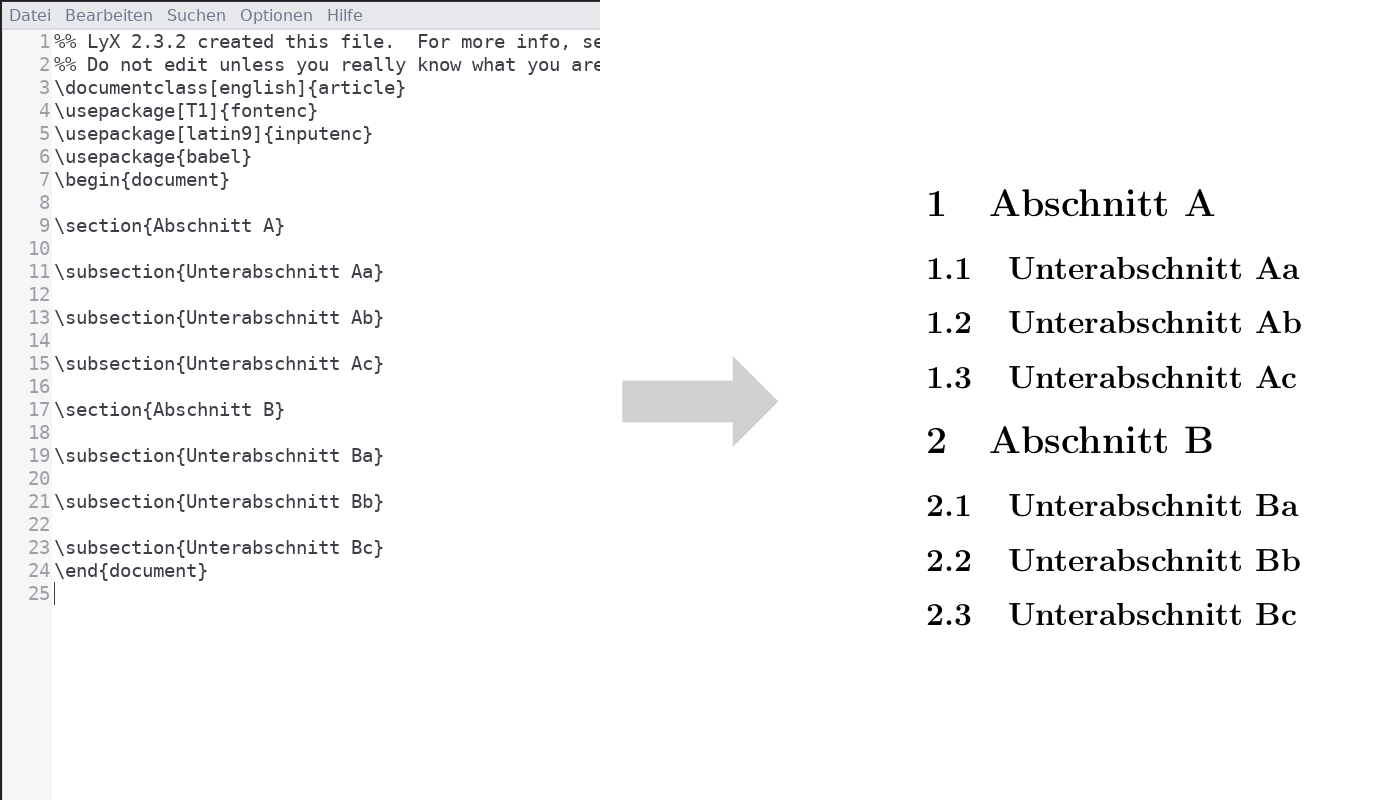
\includegraphics{image_1}\caption{\label{fig:latex-beispiel}einfacher Text mit Makros nach PDF übersetzt}
\end{figure}


\subsubsection{Installation}

\subsection{Git (Versionskontrolle)}

Diese Sektion befasst sich mit dem für Laien womöglich am schwersten
zu begreifenden Programm. Sie können sich gerne selbst bilden: \texttt{https://git-scm.com/book/de/v2}

Die Versionskontrolle ist vor allem der Grund, weshalb wir mit \TeX{}
arbeiten. Ich möchte Ihnen darlegen, weshalb es für digitale Projekte
vor allem in der Arbeitsgemeinschaft immens wichtig ist, zu versionieren.
Um nur wenige Vorteile zu nennen: 
\begin{itemize}
\item Der Arbeitsforschritt ist in einer Historie einseh- und nachvollziehbar. 
\item Der Arbeitsstand ist gesichert und kann nur mit allergrößter Mühe
verloren gehen. 
\item Mehrere Personen können gleichzeitig die Digitalisierung eines Buches
vorantreiben und ihre Arbeit zusammenfügen. 
\item Sie sehen die Änderungen/Erweiterungen Ihrer Mitstreiter. 
\item Sie können, falls etwas schief gelaufen ist, jederzeit auf alte Versionen
zugreifen. 
\end{itemize}

